\documentclass[12pt, oneside, a4paper]{article}
\usepackage{ifpdf}
\usepackage{graphicx}
\usepackage[colorlinks,bookmarksopen,linkcolor=black,pdfauthor={Sharad,Prabhakar,Vikram},urlcolor=blue]{hyperref}
\usepackage[colorlinks,bookmarksopen]{hyperref}
\begin{document}
\begin{center}
\textbf{VISVESVARAYA TECHNOLOGICAL UNIVERSITY}
\end{center}
\begin{center}
\textbf{BELGAUM}\\
\thispagestyle{empty}
\begin{figure}[htb]
\begin{center}
\ifpdf
	
\includegraphics[scale=0.50]{vtu.png}
\else
%	
\includegraphics[scale=0.50]{vtu.png}
\fi
\end{center}
\end{figure}
\textbf{SRI JAYACHAMARAJENDRA COLLEGE OF ENGINEERING}
\textbf{MYSORE-570006}\\
\textsc{department of computer science and engineering}
\end{center}
\begin{figure}[htb]
\begin{center}
\ifpdf

\includegraphics[scale=0.30]{./logo.png}
\else
%	
\includegraphics[scale=0.30]{/home/prabhakar/logo.odg}
\fi
\end{center}
\end{figure}
\begin{center}
\textbf{\underline{Project on}}\\
\textsc{Defination of our own laguage $\beta$parse\\}
\emph{\\Guidance of}\\
\textbf{P.M.SHIVAMURTHY}\\
\textit{Lecturer}\\
\textit{Dept of CS$\&$E,SJCE Mysore.}\\
\end{center}
Team:
\begin{center}
\begin{tabular}{|c|c|c|}
\hline
%% row 1
\textsc{name}
&\textsc{roll no}
&\textsc{usn}
\\\hline
%% row 2
\textsc{sharad d}
&03
&\textsc{4jc06cs089}
\\\hline
%% row 3
\textsc{prabhakar gouda}
&35
&\textsc{4jc07cs070}
\\\hline
%% row 4
\textsc{vikram tv}
&59
&\textsc{4jc07cs120}
\\\hline
\end{tabular}
\end{center}
\newpage

\newpage
\thispagestyle{empty}
\tableofcontents
\newpage
\pagenumbering{arabic}

\section{Overview}
$\beta$ - parse language is the beta version of parsing of our own language.  It involves the best possibilities that we have seen from the classic languages `C', `Scripting Languages' and others.  Language contains its own specifications for each statement.  It takes program written as per the rules and syntax of our languge as input and validates the syntax of the program and displays the result as \emph {valid} or \emph{invalid} program.In case of any error in the program the system counts number of errors as well as display the line number in which the error is detected.\\

\section{Glossary}
\begin{tabular}{ll}
%% row 1
$\beta$parse & It is our own language defined.\\
source program & User program written in $\beta$parse spec.\\
keywords & The keywords supported by our language.\\
HTML & Hyper Text Markup Language.\\
dotty & Product to support graph display.\\
kgraphviewer & Product to support graph display (kde version).\\
**.vps & Our own language extension although any extension is supported.\\
\end{tabular}

\section{References}
\begin{itemize}
\item Lex and Yacc by John R. Levine, Tony Mason, Doug Brown - O’Reilly Publications
\item A Compact Guide to Lex and Yacc by Tom Niemann at \href{http://epaperpress.com}{epaperpress.com}
\item \href{http://en.wikipaedia.org/wiki/Syntax analysis}{Wikipaedia}
\end{itemize}

\section{Requirement}
\subsection
{User requirements}
\begin{itemize}
\item System allows users to enter data from source file containing program in $\beta$parse. 
\item User can install the product by \emph{make install}.
\item Source program can be parsed using $\$$betaparse \emph{filename}
\item User can view the created parse tree by \emph{make tree}.
\item The errors are displayed by \emph{make view}. Displayed in the browser (firefox).
\item The colours are used to differentiate errors in program.
\item The product can be uninstalled by \emph{make uninstall}.

\end{itemize}
\subsection
{System requirements}
\begin{itemize}
\item Machine must run in Linux platform.
\item Machine must support Lex and YACC.
\item Machine must have the system with 256MB of RAM or better.
\item GNU C compiler (cc or gcc).
\item Machine must contain kgraphviewr or dotty for displaying the tree.
 \end{itemize}
\subsection
{Functional and domain requirements}
\begin{itemize}
\item All source files are visible to user.
\item It must display the line number of the invalid syntax in case of $\beta$parse programs.
\item The parse tree display is done using \emph{kgraphviewer} or \emph{dotty}.
\item The final validated program is displayed in \emph{html} format.
\item The different colours are used for user friendliness.
\end{itemize}
\subsection
{Non-functional requirements}
\begin{itemize}
\item Easy to use User interface.
\item Efficiency in analyzing.
\item Versatility in handling all types of C assignment source code.
\item The creation of parse tree for both error and error-free program is must.
\item The parse tree shows red colour for invalid statement in program.
\item The program may contain any extention(like *.txt, *.vps)
\end{itemize}
\section{Form Based Approach}
\textbf{Function}:\\Defination of language $\beta$parse.Checks for correctness of the program written in $\beta$parse.\\\\
\textbf{Description}:\\
Program takes input from file and analyses the syntax of the statements and returns the validity of the program.\\\\
\textbf{Input}:\\ Program defined in language $\beta$parse.\\\\
\textbf{Output}:\\Validity of the program is displayed on screen and parse tree in created for the same program.\\\\
\textbf{Action}:\\
Program is parsed. The lexical analyser searches for tokens from input stream 
and returns the token. Yacc parses the input and sets the valid bit to '0' if statement is valid else sets to '1'.The statement containing error the line number of error is displayed.The parser make call to write the file for tree.Each statement in program indicates the node in parse tree.The final program execution can be simulated by reading the leaf nodes of the parse tree.\\\\
\textbf{Requires}:\\Machine must contain Lex and Yacc packages.The kgraphviewer or dotty packages for tree display.\\\\
\textbf{Pre-condition}:\\The input file must exist in the specified path.\\

\section{Data Flow Diagram}
The data flow diagram shows that the program writen in $\beta$parse language is taken as input, which is passed to the lexical analyser.The lexical analyser returns tokes to syntax analyser.The syntax scanned by the lexar is outputed in the form of parse tree.
\begin{figure}[htb]
\begin{center}
\ifpdf
	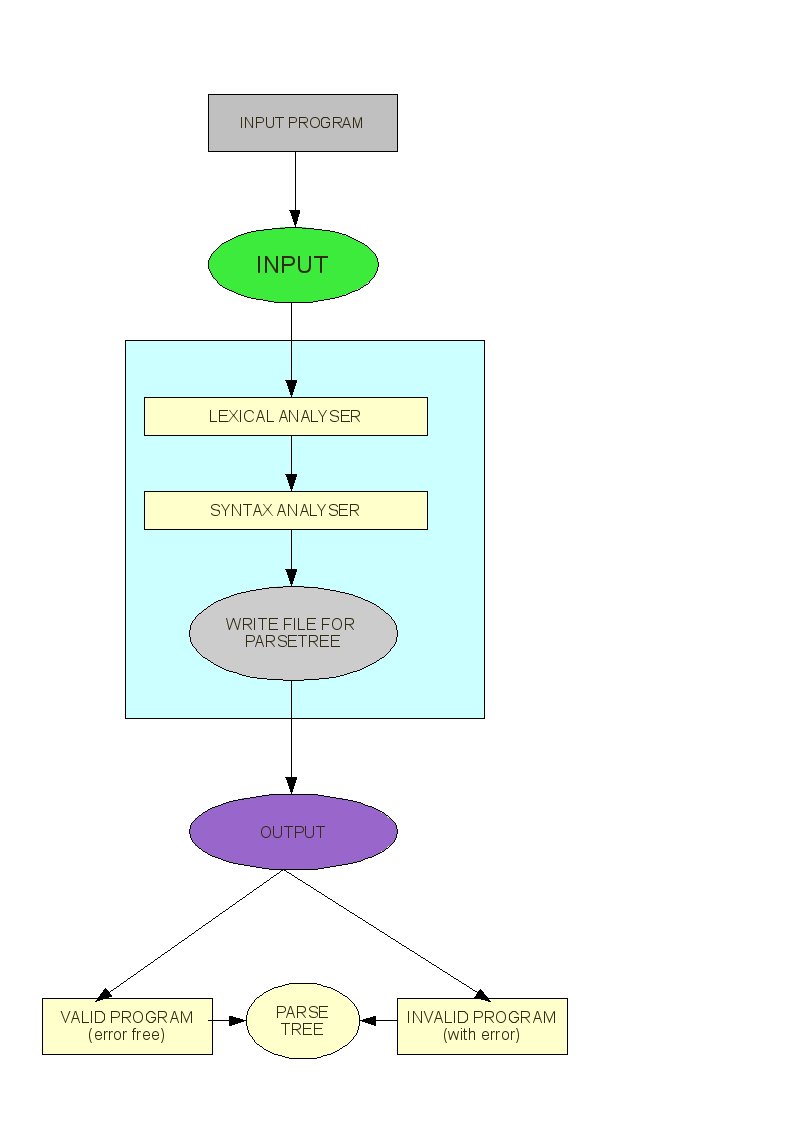
\includegraphics[scale=0.40]{DFD.png}
\else
\fi
\caption{Data Flow Diagram}
\end{center}
\end{figure}
\newpage
\section{Life Cycle}
The parser is evolved in various phases.  It is to be evolved during
\begin{itemize}
\item Requirements
\item Design
\item Implementation
\item Optimization
\item Testing
\item Installation
\item Operation and Maintenance
\end{itemize}
The product is developed making use of the \emph{spiral development model}.  Each release is updated with new functionalities and features. Development activities starts from the design phase of previously released versions.  The product is released based on user suggestions and optimizations.

\section{Constructs of the Language}
The program consists of 3 parts:
\begin{itemize}
\item The `file inclusion' part
\item The `macro definition' part
\item The `function definition' part
\end{itemize}

\subsection{File Inclusion}
File inclusion is done using the keyword \textbf{include}.\\

\hspace{.5in} \textbf{Syntax:}
	
\hspace{1in}  \textbf{include} \emph{filename}\\


Filenames should not contain any extensions.  Hence unique files are included.
The include directive can be placed anywhere in the program and every file that is to be included should in a separate line.\\

\emph{Example}: include stdio\\\\
The directive includes the file "stdio" to the current scope.

\subsection{Macro Definition}
Macro Definition has the keywords \textbf{macro} to begin the macro definition and \textbf{endm} to end the macro definition.\\

\hspace{.5in} \textbf{Syntax:}
	
\hspace{1in}  \textbf{macro} \emph{macroName code} \textbf{endm}\\

The above syntax defines a macro with name `macroName' having the body `code' and ended with keyword endm.
The macroName should not contain any special characters and its declaration is similar to the declaration of the `C' variables.
The `code' part can contain any assignments, function calls, relational condition structures, looping structures \emph{except} the function definition itself. This is to distinguish between function characters from macro characters.  The code can be spread over multiple lines.\\

The macro definitions can be included anywhere in the program but not inside any functions.

\emph{Example}: macro aIncrement a++; endm 

\hspace{1in} or

\hspace{.75in}macro aIncrement

\hspace{1in}a++;

\hspace{1.15in} .

\hspace{1.15in} .

\hspace{.75in}endm


\subsection{Function}
Function can be started by specifying the function name and parameter list for the function enclosed within parenthesis.  Every function is terminated by the keyword \textbf{endf}.\\

\hspace{.5in} \textbf{Syntax:}
	
\hspace{1in}  functionName (parameterList) \emph{body} \textbf{endf}\\

The parameter list can be zero or more.  The elements of the list should be separated by comma (,).  The function body can contain any number of basic statements like assignment, increment, decrement that resemble the 'C' statements.  The body can also include the relational operations, looping operations and function calls also.

\emph{Example}: main(argc, argv) s = p + v; a++; endf

\hspace{1in} or

\hspace{.75in}main(argc, argv)

\hspace{1in}s = p + v;

\hspace{1in}a++;

\hspace{1.15in} .

\hspace{1.15in} .

\hspace{.75in}endf

Every statement within the function body should end with a semicolon (;) similar to `C' language syntax.
The \emph{return value} of the function lies in its name only.\\

The details of the various types of statements in our language construction is dealt in the next section.

\section{Syntax of Statements}
The following are the various types of syntax that are used:

\subsection{Operators and Symbols}
The following \textbf{operators} are supported in the language.  It includes the basic arithmetic operators.\\
\begin{tabular}{ll}
+ & to perform binary addition of two variables.\\
- & to perform binary subtraction of two variables.\\
$*$ & to perform binary multiplication of two variables.\\
/ & to perform binary division of two variables.\\
, & (comma) to separate the variable declarations and also to\\ &  separate assignment statements.\\
= & to assign the rvalue obtained by an expression to the lvalue.\\
$\wedge$ & to perform the binary power operation.\\
$\%$ & to perform the modulo operation.\\
\end{tabular}
\\\\\textbf{Relational Operators:}\\
The following operators on two variables or expressions returns a boolean value.  These operators are used to test the various conditions in the language.\\\\
\begin{tabular}{ll}
== & checks for equivalence of two variables or expressions.\\
!= & checks if left variable or expression is equal to or not to the right.\\
$>$ & checks if left variable or expression is greater than to the right.\\
$<$ & checks if left variable or expression is less than or equal to the right.\\
$>$= & checks if left variable or expression is greater than or equal to the right.\\
$<$= & checks if left variable or expression is less than or equal to the right.\\
\end{tabular}
\\\\\textbf{Ternary Operators:}\\
? : Checks for the condition and assigns the value between `?' and `:' or the value after `:'.\\
\\\textbf{Structural Operators:}\\
\begin{tabular}{ll}
. & to access the members of a structure using the object (as implemented in C).\\
-$>$ & to access the members of a structure using pointer operation (as implemented in C).\\
\end{tabular}
\\\\The following \textbf{symbols} are used:\\\\
\begin{tabular}{ll}
; & to terminate a statement in the program.\\
( ) & to specify a function call and the precedence of evaluation.\\
$[$ $]$ & to specify the array related activities (similar to 'C')\\
\end{tabular}

\subsection{Variables}
The language supports all the characters (both uppercase and lowercase) of the English Language.  It also supports the integer values.  Any variable can be declared on the lines of variable declaration in 'C'.
\begin{itemize}
\item The variable can have both the characters and integers in it.
\item The variable should start with an English character and not by an integer.
\item The variable can be of any length.
\item Keywords of the language cannot be used as variables.
\end{itemize}

\subsection{Commenting}
Commenting in the language is similar to the commenting styles in C++ language.

\hspace{.5in} \textbf{Syntax:}
	
\hspace{1in}  // \emph{comment}\\

The entire line after `//' is considered as a comment and it is not parsed.

\subsection{Declaration}
The type declaration of variables used in the program are not needed and the variables can be used directly, although some of the basic datatypes (integer, float, character) are provided.  The variable is casted according to the rvalue used in the program.  Also multiple declaration of variables in a single line separated by commas are possible.  This form of declaration is inspired from the `shell scripting' language.  The declarations are to be terminated by a semicolon to mark the end.\\

The declaration of a new variable is made at its first assignment.

\emph{Example}: a = 3;\\\\
This declares the variable 'a' and assigns to it the value 3.

\subsection{Assignment}
The assignment statements are implemented based on the syntax of assignments done in 'C' Language.  The `rvalue' is assigned to the `lvalue'.  The left value can consist only one variable and not a number as a single value cannot be assigned to two or more variables on left.  The right value can consist of a variable, number or a combination of both to form a compound expression.\\

All assignment statements should terminate with a semicolon.\\

The following assignment statements are supported:\\
\begin{itemize}
\item Direct Assignment as `a = b;'
\item Compound Assignment as `a += b;'
\item Multiple Assignment (partially implement as of now) as `a = b = ... = z;'
\item Increment and Decrement as `a++;', `++a;', `a$-$$-$;' or `$-$$-$a;'.
\item Structural operational assignments (as in C) as `a-$>$node = b.leaf;'.
\item Evaluation of expressions within `( )', that has the highest order.
\item Array assignments as `a[i] = b[j];'
\item \emph{Function Calls} can also be made and the return values can be assigned as `a = hello();'.
\end{itemize}

\subsection{Relational Condition Checking - The `test-otherwise-endl' construct}
The language uses the following syntax to perform the relational condition checking.

\hspace{.25in} \textbf{Syntax:}

\hspace{.5in}  \textbf{test} \emph{condition} statements1 \textbf{endt}\\

\hspace{.5in}  or\\

\hspace{.5in}  \textbf{test} \emph{condition} statements1 \textbf{otherwise} statements2 \textbf{endt}\\

The test keyword tests for the boolean value of the condition.  The condition uses the relational operators between two variables or expressions.  If the condition is true, then the \emph{statements1} are executed.  In the second case, if the condition results false then the keyword otherwise is parsed to execute the \emph{statements2}.  The keyword endt is compulsory to mark the end of the `test-otherwise-endt' relational construct.\\

The statements1 and statements2 can inturn contain any number of nested `test-otherwise-endt' conditions.

\subsection{Looping Construct}
The looping construct is implement in the language using the keywords \textbf{loop, from, step} and \textbf{endl}.\\

\hspace{.25in} \textbf{Syntax:}

\hspace{.5in}  \textbf{loop} \emph{condition} statements \textbf{endl}\\

\hspace{.5in}  or\\

\hspace{.5in}  \textbf{loop} \emph{condition} \textbf{from} assignment \textbf{step} assignment statements \textbf{endl}\\

Looping of the \emph{statements} is done only if the \emph{condition} is satisfied.  It can also be supplement with keywords - from and step that determine the start and end of the looping.  The looping structure is finally terminated by endl keyword.\\

The statements can inturn contain any number of nested looping structures.

\subsection{Nesting of Statements}
The language supports nesting of statements.

The statements containing the `test-otherwise-endt' and `loop-from-step-endl' can be nested.  Any number of statements can be used in them.  Also the nested can be to any level in depth.  The `test' can nest `test' or `loop' or both.  Similarly, `loop' can nest `loop' or `test' or both.  The macro definitions can also nested and they may be defined anywhere in the program but between the functions.

Thus any of the \emph{nesting} combinations works well with the language.

\subsection{Program}
The language supports to have \emph{any number of} `functions', `macros', `file inclusions', `conditional executions', `looping constructs' and `statements' in the program.  Each construct is supposed to be terminated by appropriate terminator.  Finally the program itself needs to be terminated by the keyword \textbf{endp}.

\newpage
\section{Design of Parser}

The source program contains our language.  The parser checks the source program for errors, that is identifies which part in the source program has deviated from our language specification.  It finally output the errors.

\subsection{Architectural Design}
The design involves identifying the different tokens and keywords of the language and integrate them with rules that are specified in the language specification.  

\begin{figure}[htb]
\begin{center}
\ifpdf
	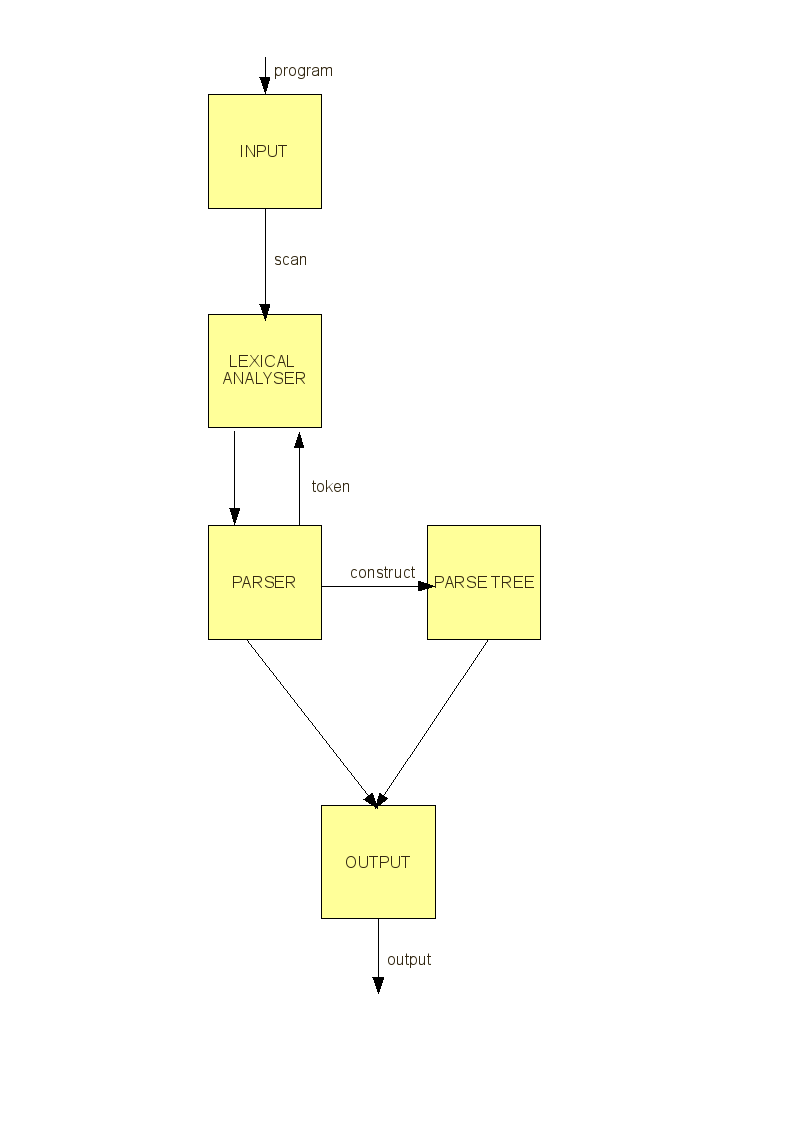
\includegraphics[scale=0.40]{design.png}
\else
\fi
\caption{Design Process}
\end{center}
\end{figure}

\subsubsection{System Organisation}
The source file can be accessed by the tokens and keywords indentifier \emph{and} also by the grammar checker.  Hence a shared data repository model is feasible.  The shared data here is the source program.

\subsubsection{Modules}
One module needs to fetch the keywords and tokens that are defined in the language.  The other module receives the tokens and keywords and checks for the grammar required by the language.  The `lexer' does the job of fetching the keywords and token from the source program and the `parser' does the job of handling them to match the grammar as specified by the language.  If the grammar is violated, then the source program is not in our language specification and an error message is outputted.  If an error is found in the source file, then the line number of error occurence from source file is outputted and the grammar checking continues with the entire source file.

\subsubsection{Cohesion}
The modules are interconnected by a common buffer storage area.  The lexer identifies and loads the keywords and tokens from source file to a buffer which is also referred to by the parser.

\subsection{Detailed Design}
The current design consists of few tokens and keywords.  The lexer identifies the following tokens and keywords from the source file.\\
\begin{itemize}
\item It can identify the keywords - test, otherwise, endt,  loop, from, step, endl, include, macro, endm, endf, endp, //
\item It can also identify the variables, numbers, operators, symbols and newline character.
\end{itemize}
The parser checks for the following grammars.
\begin{itemize}
\item Check for expression.  An expression can consist of left and right parts.\\
Left part can have only a single variable.  Right part can have variables, numbers or both forming compound statements.\\
The grammar could be something as\\

expression : left right\\
left : variable\\
right : autoIncrementandDecrement ;
\hspace{.75in}$|$ variable operators variable ;
\hspace{.75in}$|$ ([variable $|$ right]) ;\\

\item The assignment statements are then identified at a higher level that may consists of the expression or the auto increment and decrement operations or the datatype declarations or the compound assignments.  It can be as\\
assign : autoIncrementandDecrement $|$ multipleAssignments

\hspace{.5in}$|$ termination $|$ assign ;\\
autoIncrementandDecrement : variable autoOperation

\hspace{2in} $|$ autoOperation variable\\
autoOperation : ++ $|$ $-$$-$\\
\item The function calls in the language could be as\\
functionCall : variable ([parameters])\\
parameters: variable $|$ parameters , variable\\
The parameters inside [ ] indicate that it is optional.\\
\item The relational condition checking `test-otherwise-endt' is implemented:\\
relCond : test condition statement endl

\hspace{.5in} $|$ test condition statement otherwise statement endl\\

The condition and statement are defined in the next sections.\\

\item The looping construct is implemented as\\
loopcond : loop condition statement endl

\hspace{.5in} : loop condition from assign step assign statement endl\\

\item Implementing `condition':\\
condition : variable [==, !=, $>$, $<$, $>$=, $<$=] variable\\
The conditions can be any of the relational conditions given within [ ].\\

\item Implementing `statements':\\
statement:	assign

\hspace{.75in}$|$	relCond $|$	loopCond 

\hspace{.75in}$|$	funcCall ;

\hspace{.75in}$|$	statement assign

\hspace{.75in}$|$	statement funcCall ;

\hspace{.75in}$|$	statement relCond

\hspace{.75in}$|$	relCond statement

\hspace{.75in}$|$	statement loopCond

\hspace{.75in}$|$	loopCond statement

\item The file inclusion, macro and function can be implemented as:\\
include : include variable\\
macro : macro variable code endm\\
func : functionCall code endf\\

\item The recursive call in the program is implemented using the `code', `parts' and `program' as:\\
code : statement $|$ relCond $|$ loopCond

\hspace{.5in}$|$ code statement $|$	code relCond $|$	code loopCond\\

parts : include $|$ macro

\hspace{.5in}$|$ include macro $|$ parts include $|$ parts macro\\

program : parts $|$ program parts

\hspace{.5in}$|$ func $|$ parts func $|$ program func\\

\item Finally the entire program is ended with the keyword `endp' and the implementation is\\
full : program endp\\
If the above rule is satisfied then the source program contains no errors.  Otherwise the errors that occur in between are to be outputted with linenumber.
\end{itemize}

\subsection{Interface Design}
\begin{itemize}
\item The tokens and keywords are scanned by the lexer and put into a buffer.  The parser requests for a particular token at which the lexer starts scanning the tokens.  The tokens put into the buffer by the lexer are picked up the parser for grammar checking.

\item During the course of grammar checking, if an error is encountered the particular linenumber from the source program is outputted.
The line numbers with errors are further stored into an array `errorlines'.

\item In order to display the error lines from the source file, the `errorlines' are sent to the display function.  The error lines are then recognized and displayed suitably.

\item Parse tree is constructed by referring to the line numbers containing the errors and formatted to the .dot format.
\end{itemize}


\section{Example Program}
The following screenshot example shows the usage of the \emph{betaparse}.\\
The test code is given in the figure `Code'.\\
The executing of the code using betaparse is shown in `Terminal'.\\
The parse tree that is generated is shown in `Parse Tree'.\\
The error lines are differentiated from source program in `HTML Error View'.

\begin{figure}[htb]
\begin{center}
\ifpdf
	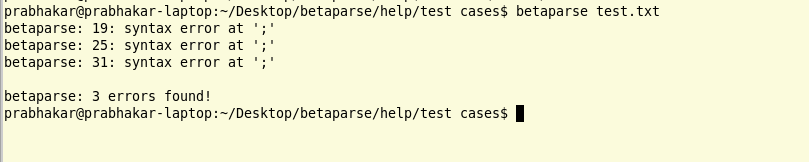
\includegraphics[scale=0.50]{example1.png}
\else
%	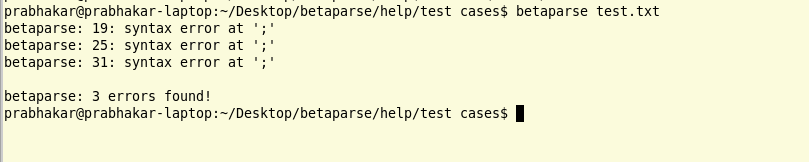
\includegraphics[scale=0.50]{example1.png}
\fi
\caption{Terminal}
\end{center}
\end{figure}
\newpage
\begin{figure}[htb]
\begin{center}
\ifpdf
	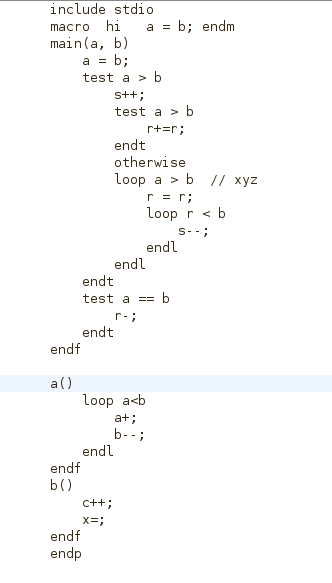
\includegraphics[scale=0.70]{example.png}
\else
\fi
\caption{Code}
\end{center}
\end{figure}

\newpage
\begin{figure}[htb]
\begin{center}
\ifpdf
	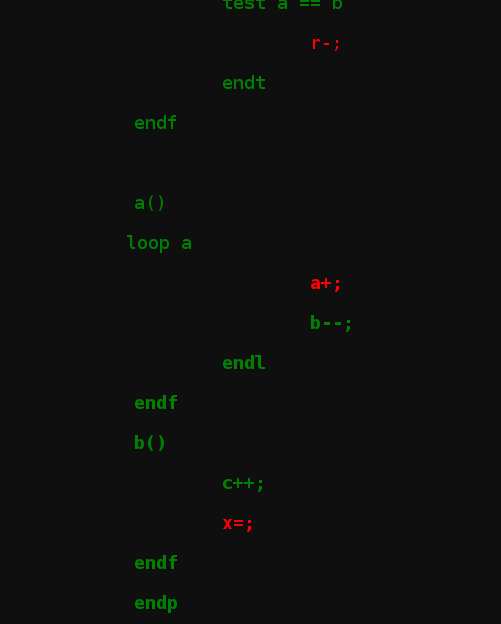
\includegraphics[scale=0.60]{example3.png}
\else
\fi
\caption{HTML Error View}
\end{center}
\end{figure}

\begin{figure}[htb]
\begin{center}
\ifpdf
	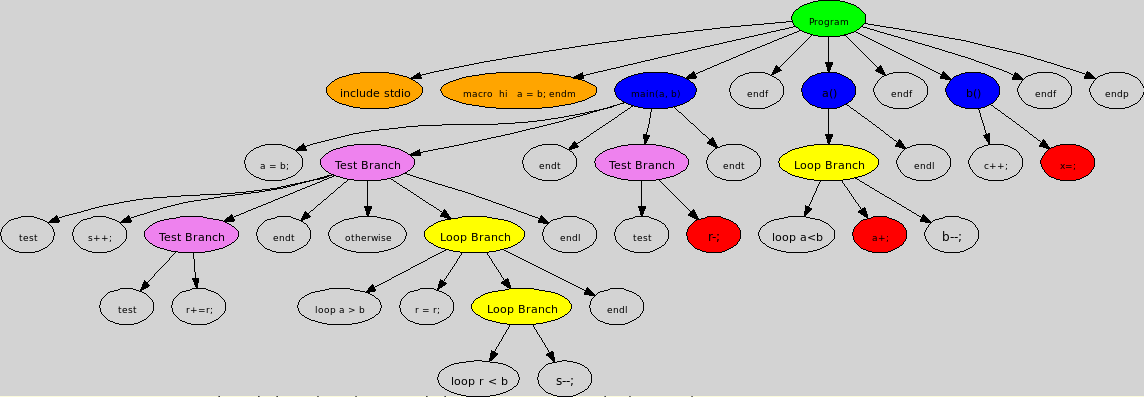
\includegraphics[scale=0.50]{parsetree.png}
\else
\fi
\caption{Parse Tree}
\end{center}
\end{figure}
\newpage 
\section{Final Deliverable}
\begin{itemize}
\item Archive of Product with Source code.
\item Documentation.
\item File containing suitable test cases.
\end{itemize}

\section{Applications}
\begin{itemize}
\item The designed $\beta$parse can be effectively used to verify the syntax of most of the possible programs written in $\beta$parse syntax.
\item Can be used to simulate the\emph{parse tree} creation.
\end{itemize}


\section{Future Work}
\begin{itemize}
\item The number of tokens and keywords currently supported are to be increased in future releases.
\item Further evolve the current version of `parse tree' implementing terminals for each tokens in the language.
\item Implementing \emph{auto make} and \emph{auto configure} before installation.
\item Develop a compiler that supports our language $\beta$parse and the needed optimizations.
\end{itemize}

\section{Conclusion}
Syntax analyzer is the major module used in any compiler. By repeated testing, we have found out that syntax analyser for $\beta$parse program statement successfully analyses and provides an easily understandable interface for the user to interact with system.  The syntax that are to be followed in the language are simple with most them beign English statements and less number of brackets and datatype declarations.  The language currently supports \emph{any number} of file inclusions, macros, functions, loop and conditional structures and statements of various types.  The syntax errors are successfully found. The expected results have been obtained and hence the implementation of the Syntax analyzer for $\beta$parse has been found successful.
\end{document}
